\documentclass[9pt]{sigplan-proc-varsize}
%\documentclass[noindentedparagraphs]{sigplan-proc-varsize}



% % hack to avoid the ugly ACM paragraph definition
% % => can't leave blank line after this
% (remove comment for this hack)
% \renewcommand{\paragraph}[1]{\vskip 6pt\noindent\textbf{#1 }}

\usepackage{graphicx}
\usepackage{url}
\usepackage{sidecap}


\numberofauthors{2}


\author{
%
% The command \alignauthor (no curly braces needed) should
% precede each author name, affiliation/snail-mail address and
% e-mail address. Additionally, tag each line of
% affiliation/address with \affaddr, and tag the
%% e-mail address with \email.
\alignauthor Ankit Goyal\\
        \affaddr{Department of Computer Science}\\
        \affaddr{University of Texas at Austin}\\
       \email{ankitgoyal@utexas.edu}
\alignauthor Sreedevi Surendran \\
    \affaddr{Department of Computer Science}\\
    \affaddr{University of Texas at Austin}\\
    \email{sreedevi@cs.utexas.edu}
}

\title{Power Aware HTTP: Modifying HTTP to optimize power consumption}

%
% stock conference info---get from the publisher
%
%\conferenceinfo{SenSys'06,} {November 1--3, 2006, Boulder, Colorado, USA.}
%\CopyrightYear{2006}
%\crdata{1-59593-343-3/06/0011}

\newlength\myindent
\setlength\myindent{1em}
\newcommand\bindent{
  \begingroup
  \setlength{\itemindent}{\myindent}
  \addtolength{\algorithmicindent}{\myindent}
}
\newcommand\eindent{\endgroup}

\newlength\mysecindent
\setlength\mysecindent{2em}
\newcommand\quadindent{
  \begingroup
  \setlength{\itemindent}{\mysecindent}
  \addtolength{\algorithmicindent}{\mysecindent}
}
\newcommand\quadeindent{\endgroup}


\begin{document}

\special{papersize=8.5in,11in}
\setlength{\pdfpageheight}{\paperheight}
\setlength{\pdfpagewidth}{\paperwidth}


\maketitle


\begin{abstract}
\noindent A major part of the Internet works on the HTTP protocol. Optimizations to the protocol have been suggested to improve the performance of the protocol. However, less attention has been paid to the power consumption aspect of the protocol which is bound to play a significant role in the coming years due to an increase in mobile devices which are constrained by limited power capabilities. In this paper, we first analyze where exactly the power is consumed, how configuration changes affect power consumption and then we propose a noval solution to reduce the power consumed by HTTP without compromising on performance. 
\end{abstract} 

%
% the following three things (cateogry, terms, keywords) are required by acm:
%

% A category with only the three required fields
\category{H.4.m}{HTTP Protocol}{Miscellaneous}
\category{D.2}{Power}{Power aware http}
%A category including the fourth, optional field follows...
\category{D.2.8}{Power aware http}{Metrics}[power consumption measures,
performance measures]

\terms{http, power-aware, optimization, network protocol}

\keywords{power aware http, network protocol}

\medskip

\section{Introduction}
  \label{sec:intro}

\medskip

The field of wireless communication has seen tremendous progress in recent years. Mobile devices are on the increase and being connected to the internet while on the move is essential in today’s society. One of the greatest constraints to realizing this goal is finite power supply which leads to short continuous operation time of mobile devices.

In this context, we first try to pinpoint the part of the HTTP protocol which leads to power consumption. We then make changes to the configurable server side properties including timeout, keepalive values etc. to analyze the level of impact these parameters have on the power consumption and finally, propose a power aware HTTP protocol that can optimize the power consumption of HTTP.

The rest of this paper is organized as follows: Section 2 highlights the background and related works of hypertext transfer protocol, transmission control protocol and power consumption issues over HTTP. Section 3 highlights the motivation behind this paper. Section 4 presents our proposed implementation of a power aware HTTP. Section 5 outlines the challenges faced during the course of the implementation. Section 6 outlines the results of our implementaion. Section 7 lists some other optimizations to optimize the power consumption of HTTP. Section 8 discusses related works. Section 9 includes our concluding remarks. Section 10 discusses the future work in the context of power optimziation of HTTP. Section 11 lists the references.

\medskip

\section{Background}

\medskip

In this section we give a brief overview of the HTTP protocol. This is followed by an overview of the connection establishment and teardown in TCP. We then discuss the inefficiencies in the HTTP protocol as it is implemented today and the power consumption observed in HTTP.

\subsection{HTTP Protocol Overview}

The HTTP protocol follows a client server model where a request (in simple ASCII format) is sent from the client to the server, followed by a response (in simple ASCII format) sent from the server to the client. An HTTP request includes the following elements: a method which can be either GET, PUT, POST, DELETE etc; a set of headers which specifies the type of content the client is ready to accept, authentication data etc; a payload field to hold data for PUT method etc. The server processes the request and sends a response to the client. The response includes a status code that indicates whether the request was successful or not and if not, the errors in the request are returned. The response also includes information about the data returned by the server like content-length of the response and the output generated by the server-side script (can be an HTML/ XML/JSON file etc). 

HTTP utilizes TCP for reliable transfer of information over the internet. To analyze the power consumption model of HTTP, it is relevant to give a brief overview of the TCP connection establishment and teardown.

\bigskip

\subsection{TCP Protocol Overview}

\subsubsection{Connection Establishment}

For a client to establish a TCP connection with a server, the client must send a SYN and receive an ACK for it from the server. Thus, conceptually, there should be four control messages passed between the devices. However, it's inefficient to send a SYN and an ACK in separate messages when one could communicate both simultaneously. Thus, in the normal sequence of events in connection establishment, one of the SYNs and one of the ACKs is sent together by setting both of the relevant bits (a message sometimes called a SYN+ACK). This makes a total of three messages, and is called a three-way handshake.

\subsubsection{Connection Teardown}

Each side terminates its end of the connection by sending a special message with the FIN (finish) bit set. This message, sometimes called a FIN, serves as a connection termination request to the other device, while also possibly carrying data like a regular segment. The device receiving the FIN responds with an acknowledgment to the FIN to indicate that it was received. The connection as a whole is not considered terminated until both sides have finished the shut down procedure by sending a FIN and receiving an ACK.

Thus, termination isn't a three-way handshake like establishment: it is a pair of two-way handshakes. The states that the two devices in the connection move through during a normal connection shutdown are different because the device initiating the shutdown must behave differently than the one that receives the termination request. In particular, the TCP on the device receiving the initial termination request must inform its application process and wait for a signal that the process is ready to proceed. The initiating device doesn't need to do this, since the application is what started the ball rolling in the first place.

\bigskip

\subsection{Inefficiencies of HTTP}

The HTTP protocol as it is implemented today has some notable inefficiencies. Explicit calls to the server are required to fetch individual resources on a webpage. Every such call requires the setup of a new TCP connection. (In HTTP/1.0, a new conenction is established on every subsequent request). This increase in the number of calls to the server adds to the power consumption and latency. Modern browsers try to  optimize this problem by maintaining "persistent" connections and pipelining requests. Also, HTTP does not  impose any requirements on data compression.

\bigskip

\subsection{Persistent HTTP Connections}

Since the TCP specification requires the host that closed/terminated the connection to retain information about that connection for four minutes [3], a client (unnecessarily) remains in a high power consumption state longer than required. However, opening and closing fewer number of TCP connections reduces processing overhead, which leads to a reduction in power consumption. We need to find an optimal time period to keep the TCP connection open given variables like content-length of the data being exchanged. 

Persistent TCP connections are enabled by default in HTTP/1.1 and is based on the HTTP keep-alive header field. Power consumption is notably optimal in case of 802.11 networks. In the case of cellular connections, the radio remains at a higher power state during the keep-alive time and is not as optimal.

\bigskip

\subsection{ Non Persistent HTTP Connections}

In the case of non persistent HTTP connections, since the client sets up a new TCP connection for every HTTP request, there are some notable inefficiencies: 

1. A typical web page consists of lot of images and text, and according to the current implementation of HTTP protocol, all the resources are fetched using a different HTTP connection which increases the number of round trips. Each round trip requires allocation of new resources such as port numbers, bookkeeping data structures, etc.

2. Increase in the number of allocated resources requires more processing power.

3. Due to TCP’s slow start approach to avoid network congestion [2], the available network bandwidth for the first few roundtrips of a connection are not utilized. TCP does not reach full throughput until the effective congestion window size is at least the product of the round-trip delay and the available network bandwidth [1]. This means that slow start limits TCP throughput, which leads to more roundtrips and consequently higher power consumption.

Non-persistent TCP connections are enabled by default in HTTP/1.1 and is based on the content-length header field.

\bigskip

\subsection{Power Consumption in HTTP}

\begin{figure}[ht!]
\centering
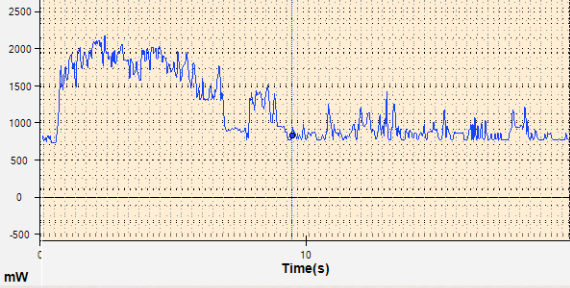
\includegraphics[width=80mm]{powerconsumption1.png}
\caption{Persistent HTTP Connection }
\label{fig:sp_gd_mnist}
\end{figure}

\begin{figure}[ht!]
\centering
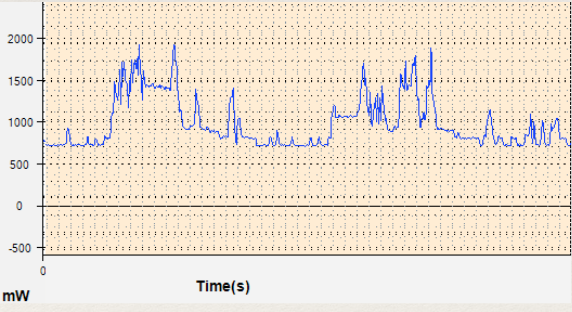
\includegraphics[width=80mm]{powerconsumption2.png}
\caption{Non-Persistent HTTP Connection }
\label{fig:sp_gd_mnist}
\end{figure}

\bigskip

\section{Motivation}

The effect of an increase in the number of calls to the server is more severe in resource-constrained devices. Since the power consumption increases with the number of requests made, we focus on novel methods to reduce the number of HTTP requests made by a webpage.

Today, conditional HTTP requests are used by clients to fetch individual resources on a webpage.  {\it If-Modified-Since} and {\it If-None-Match} are the two headers used to achieve conditional HTTP requests. Using {\it If-Modified-Since}, if the requested variant has not been modified since the time specified in this field, an entity will not be returned from the server; instead, a 304 (not modified) response will be returned without any message-body. Using {\it If-None-Match}, a client that has one or more entities previously obtained from the resource can verify that none of those entities is current by including a list of their associated entity tags in the If-None-Match header field.

In HTTP/1.1, to load a cached webpage, the number of conditional GET requests equals the number of resources. For resources that are not modified often, this is an unnecessary overhead.

We conducted a study by making web requests to some well-known and oft-visited websites. Unsurprisingly, we found that most of the resources on most of these cached webpages were seldom modified. Nevertheless, unnecessary HTTP calls were being made to attempt to fetch them again from the server.

\begin{figure}[ht!]
\centering
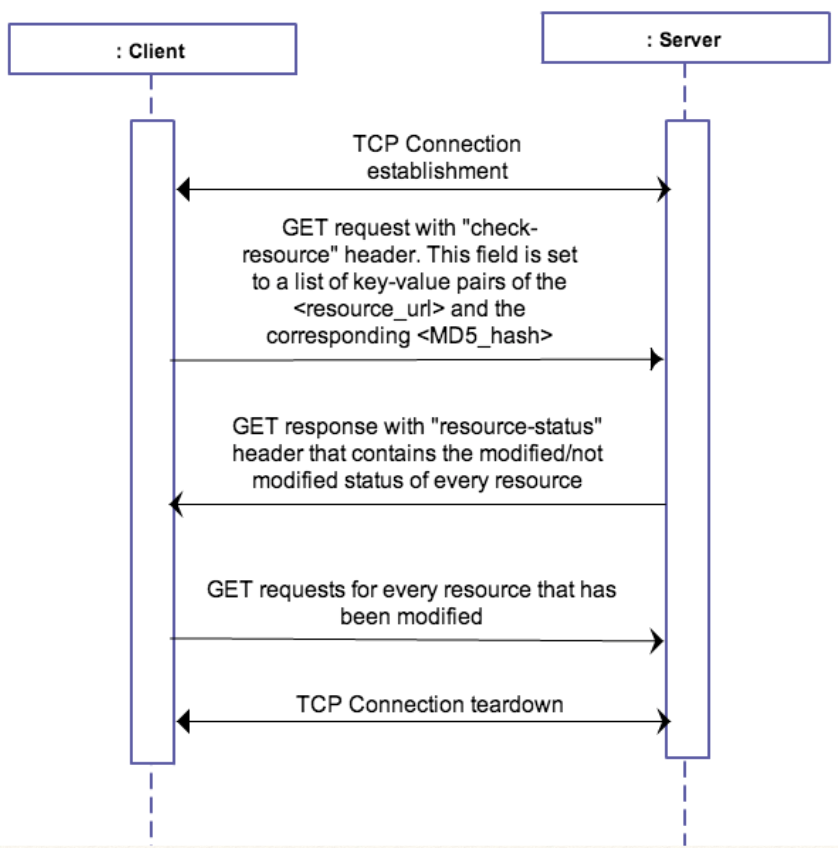
\includegraphics[width=80mm]{proposal}
\caption{Persistent HTTP Connection }
\label{fig:sp_gd_mnist}
\end{figure}

For a page that is loaded from the cache, we propose an extension to HTTP which involves the addition of two new header fields to the HTTP GET request method. {\it check-resource} in the request header would enable the MD5 hash values for multiple resources to be set by the client. {\it resource-status} in the response header would enable the server to send a bitmap containing the status of resource change.

With the extension in place, when a cached webpage is to be loaded, a single GET request will be made which will contain the MD5 hash of all the resources on the page. The server uses MD5 hash to match resources and checks whether the resources have been modified (one-by-one) and returns the status (modified/not modified) for every resource to the client. The client then makes GET requests for only the resources that have been modified.

\begin{SCfigure}
  \centering
  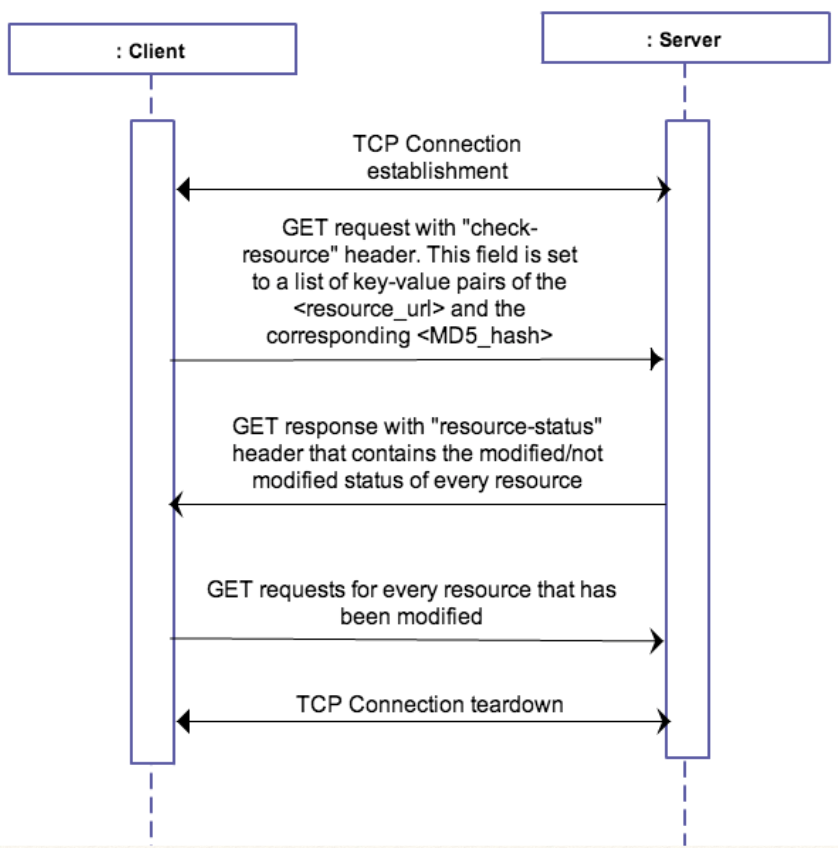
\includegraphics[width=0.5\textwidth]
    {proposal}% picture filename
  \caption{ Proposal  }
\end{SCfigure}



\begin{SCfigure}
  \centering
  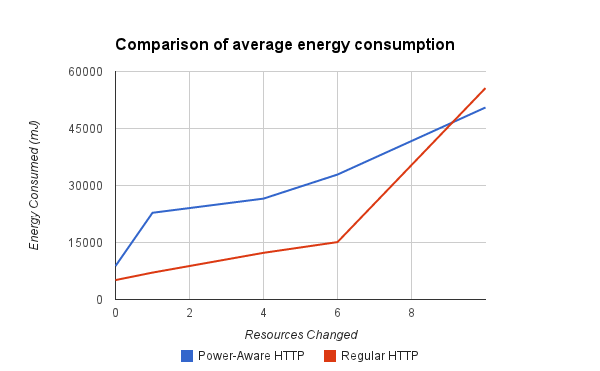
\includegraphics[width=0.5\textwidth]
    {avg_energy.png}% picture filename
  \caption{ Without Headers (Cellular)  }
\end{SCfigure}



\bigskip

\section{Implementation}

We implemented our proposal at the application layer, over both wifi as well as a cellular network (3G).

\subsection{Client}

An additional header field {\it check-resource} is added to the single GET request made by the client. 
The value of this field will be set to a list of key-value pairs of the resource-url and the corresponding MD5 hash.  When the client receives the modified/not modified status of the individual resources from the header of the response from the server, it will then make GET requests for only those resources that have not been modified.

\begin{figure}[ht!]
\centering
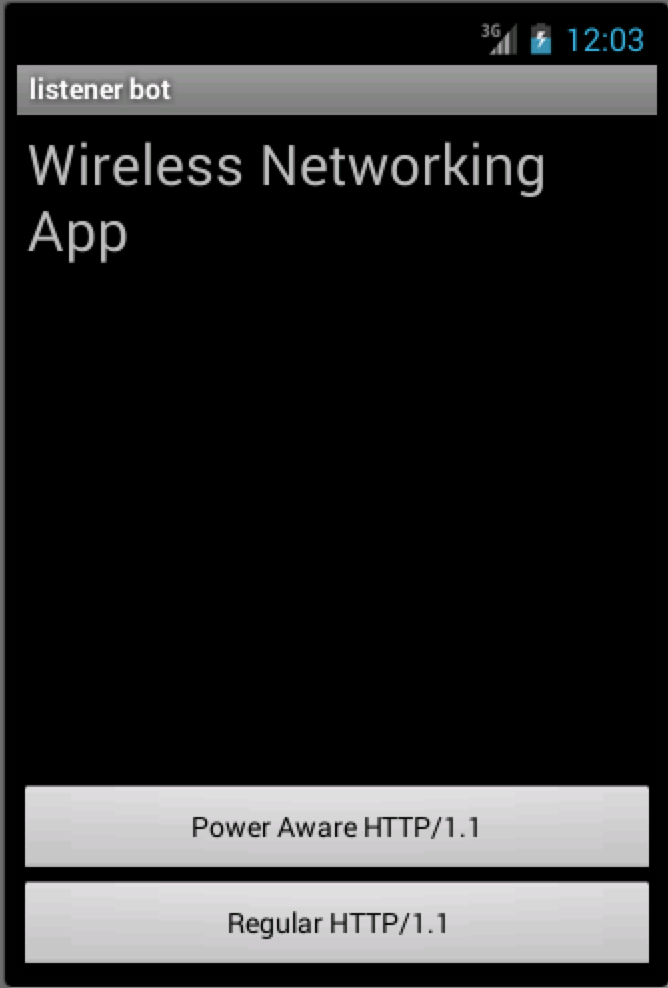
\includegraphics[width=50mm]{app2}
\caption{Client Application }
\label{fig:sp_gd_mnist}
\end{figure}

\bigskip

\subsection{Server}

The server responds with an additional response header {\it resource-status} which is a bitmap containing the modified/not modified status of every resource on the webpage.

\bigskip

\subsection{Technical Setup}

The components used for the implementation are listed below.

\subsubsection{Hardware}

\noindent1. Power Monitor by Monsoon Solutions. \newline
2. Mobile Device: HTC desire one running Android 4.2.2

\subsubsection{Software}

1. Application: Native android application

2. Servers: Apache Tomcat, Web-brick

3. Framework: Sinatra

4. Analysis: Matlab

5. Browser: Readings were also taken using Google Chrome and Firefox

\begin{figure}[ht!]
\centering
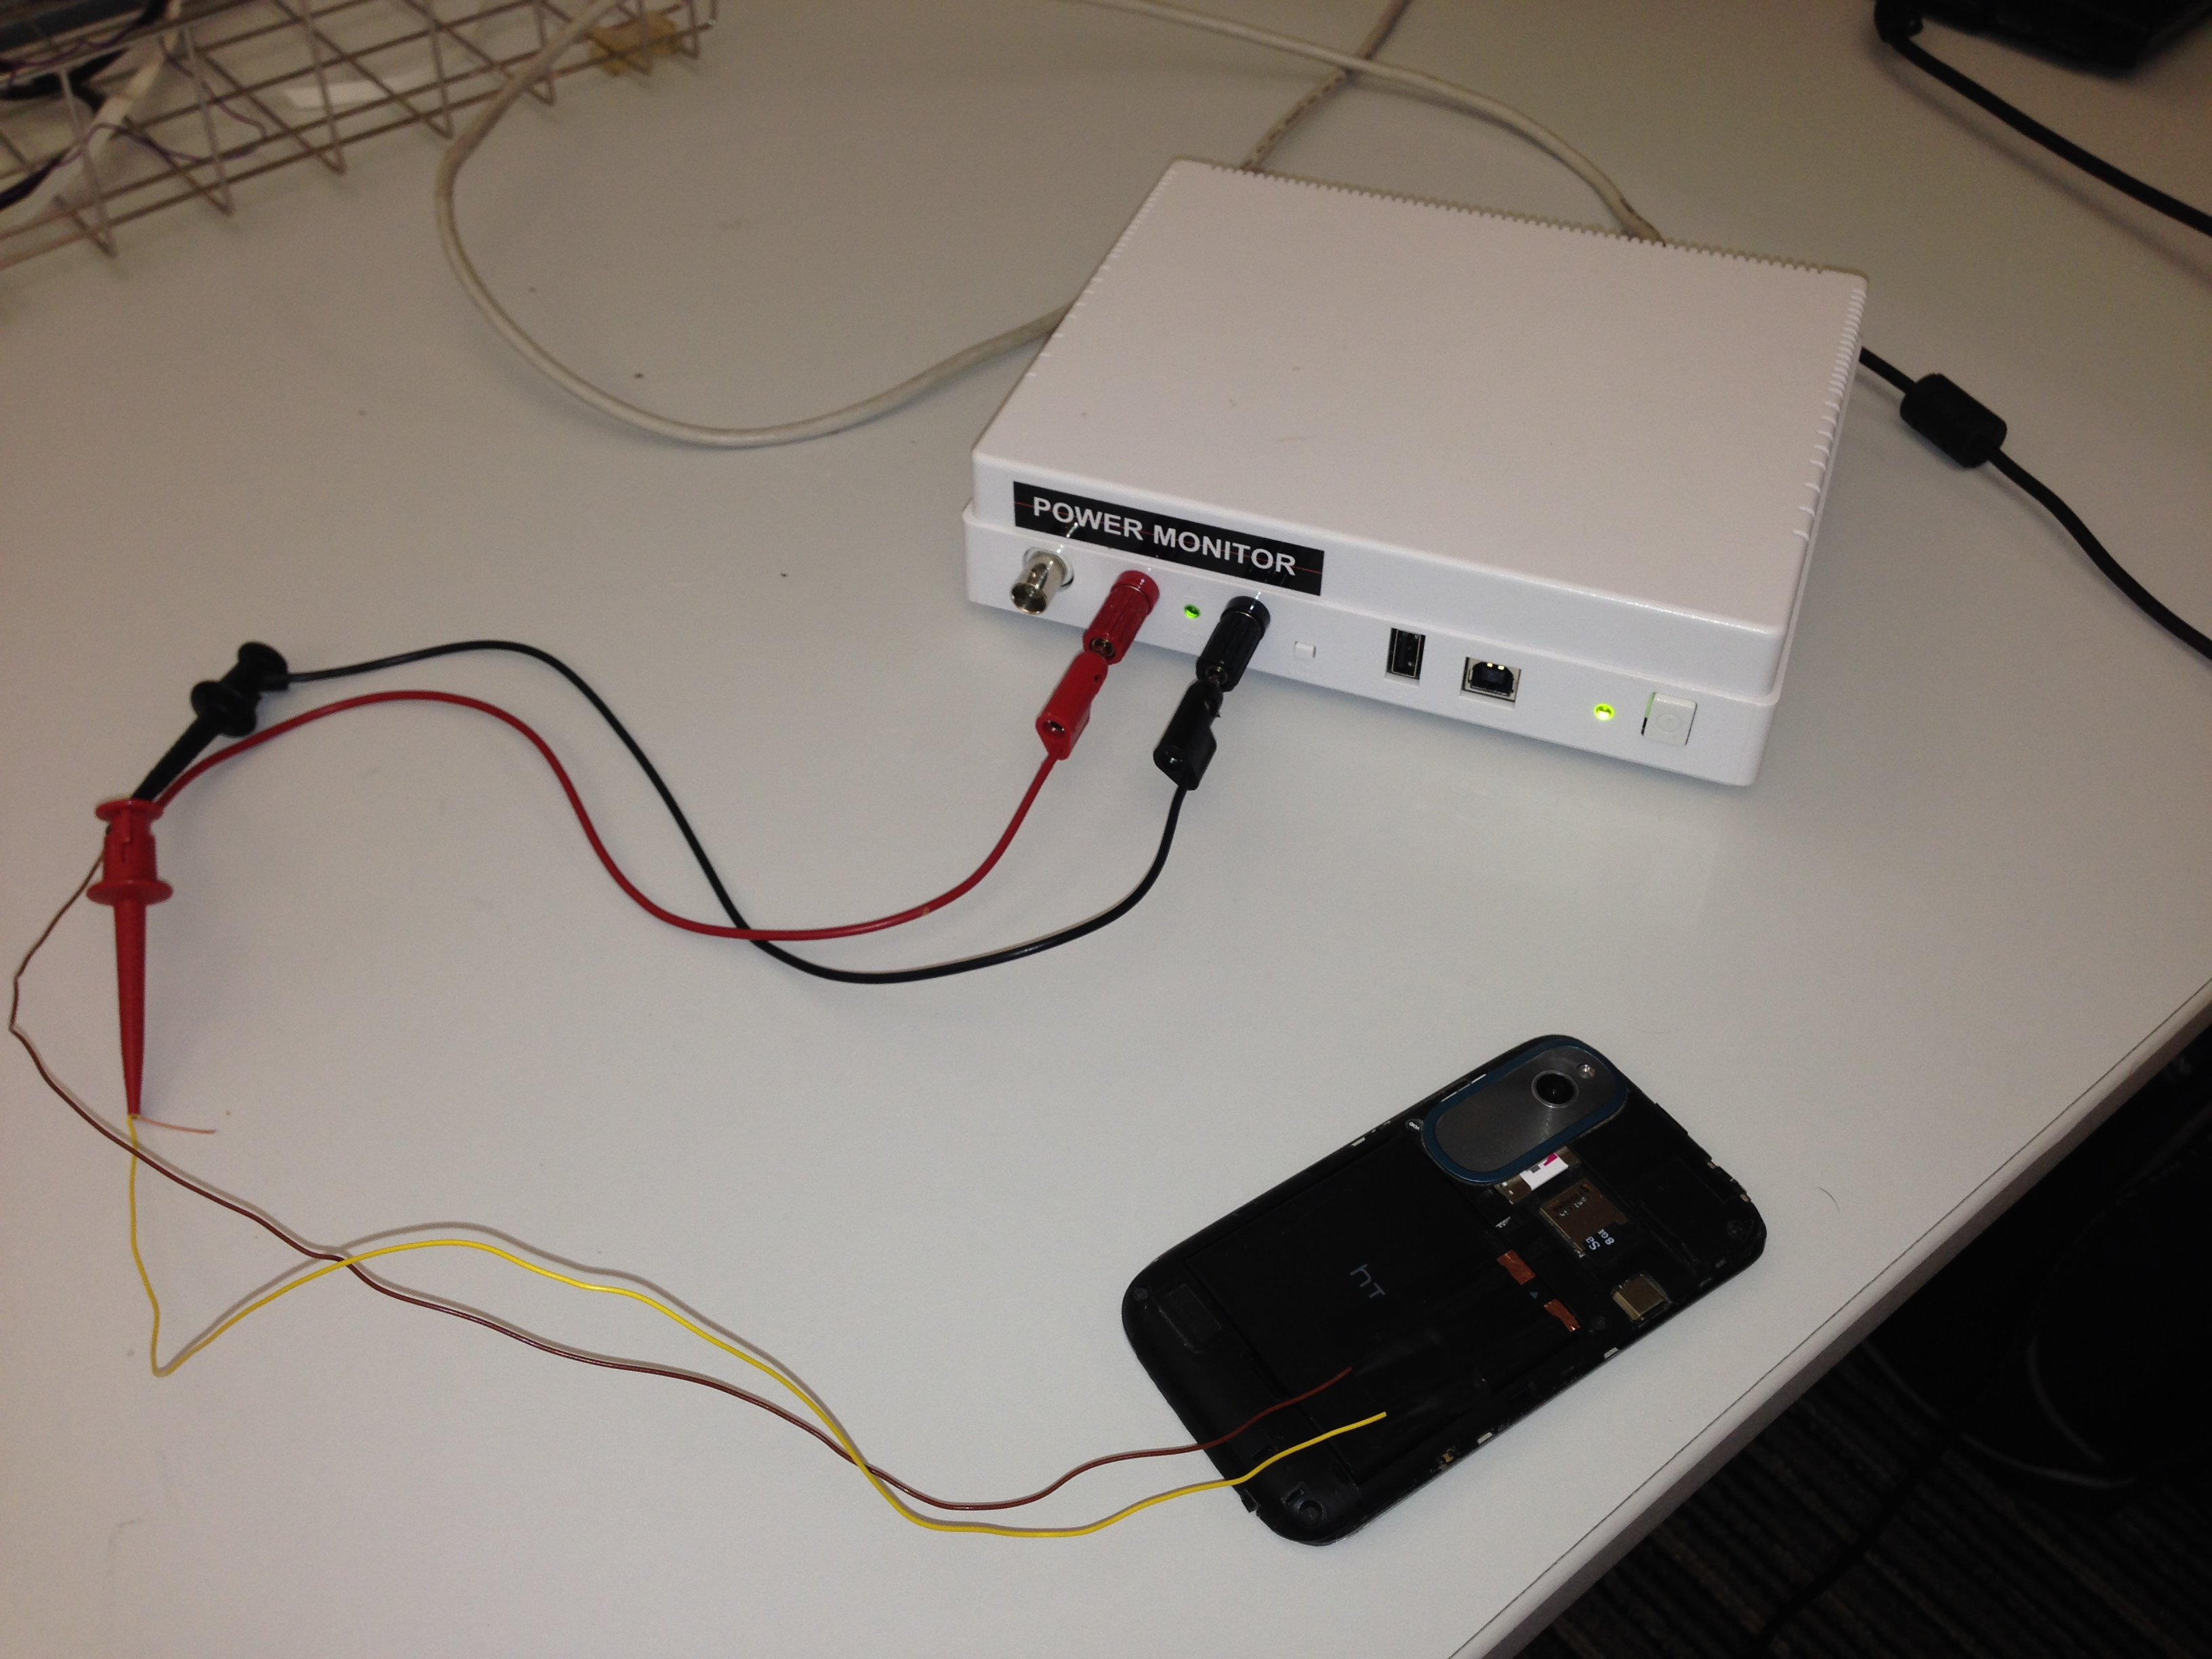
\includegraphics[width=70mm]{monitor.jpg}
\caption{Monsoon Solutions’ Power Monitor and PowerTool software were used to capture power measurements for HTTP interactions on the Android device. }
\label{fig:sp_gd_mnist}
\end{figure}

\bigskip

\begin{table}[htbp]
\caption{Power consumption in mJ for different HTTP implementations.}
\begin{tabular}{|r|r|r|r|}
\hline
\multicolumn{1}{|l|}{} & \multicolumn{1}{l|}{Power-Aware HTTP} & \multicolumn{1}{l|}{Regular HTTP} & \multicolumn{1}{l|}{Difference} \\ \hline
0 & 8813.55 & 5109.29 & 3704.26 \\ \hline
1 & 22819.33 & 7077.08 & 15742.25 \\ \hline
4 & 26546.05 & 10279.8 & 16266.25 \\ \hline
6 & 32878.45 & 15107.92 & 17770.53 \\ \hline
10 & 50532.2 & 55641.49 & -5109.29 \\ \hline
\end{tabular}
\label{}
\end{table}

\section{ Challenges}

While measuring power for different HTTP requests, a lot of spikes were observed in the power consumption graph which were not related to HTTP, since the connection was either in an idle state or the HTTP request had been completed. These could have happened due to the following reasons: 

a) Different browsers have different power consumptions and have different scheduling policy to fetch the results. For example, Google Chrome starts fetching a page as soon as you start typing the URL which may require additional processing and thus add to the power consumption.
Solution: To address this, we created an Android app that allowed us to make HTTP calls with custom headers for various scenarios eliminating any power consumption due to rendering or other optimizations. All the HTTP connections were reused and the persistence of a connection was controlled from the server side by setting the KeepAlive flags.

b) There are lot of background processes in an Android device that consume power and it becomes difficult to know whether the power spikes are due to the monitored HTTP calls or due to other processes in the system.
Solution: To alleviate the effect of other applications, we considered the average power consumption during the same fixed interval of time. We also subtracted the baseline from the origina signal to mitigate the effects of continuously running background processes. We applied the Butterworth low-pass filter to mitigate the interference of high frequency noise.

\bigskip

\section{Results}

\subsection{Measurements}

\begin{figure}[ht!]
\centering
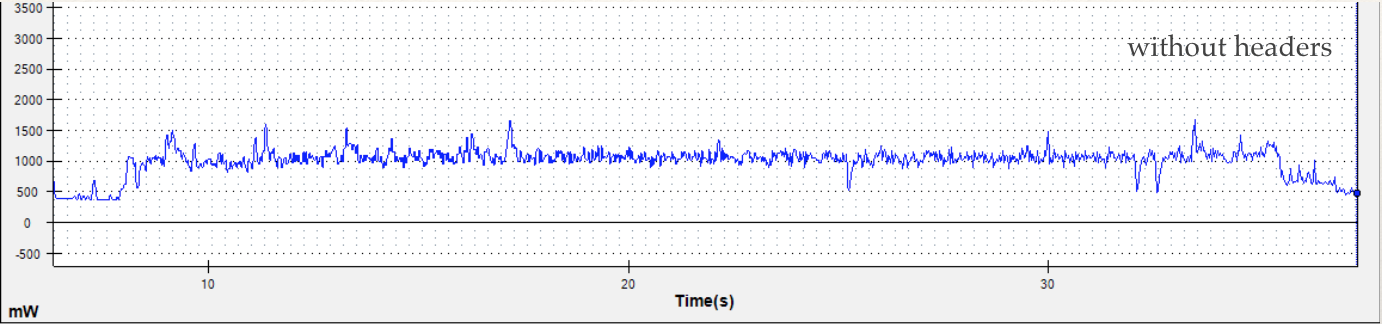
\includegraphics[width=80mm]{cellular_withoutheaders.png}
\caption{Without Headers (Cellular) }
\label{fig:sp_gd_mnist}
\end{figure}

\begin{figure}[ht!]
\centering
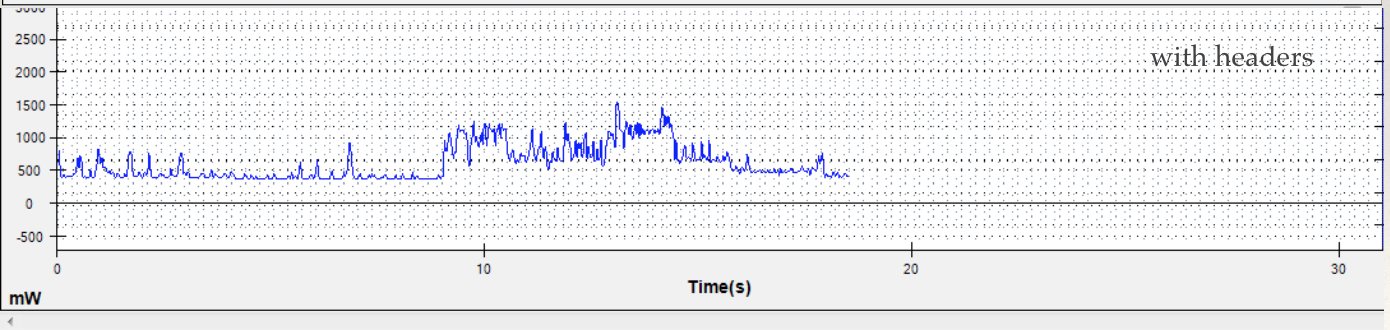
\includegraphics[width=80mm]{cellular_withheaders.png}
\caption{With Headers (Cellular) }
\label{fig:sp_gd_mnist}
\end{figure}

some text here

\begin{figure}[ht!]
\centering
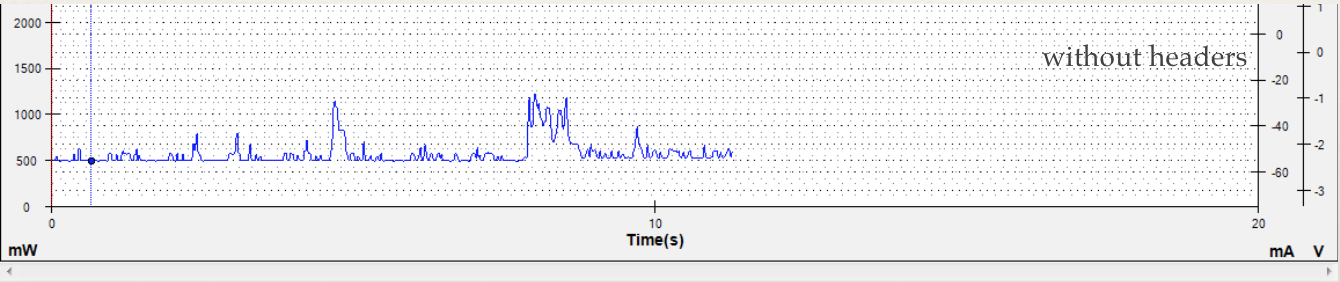
\includegraphics[width=80mm]{wifi_withoutheaders.png}
\caption{Without Headers (Wifi) }
\label{fig:sp_gd_mnist}
\end{figure}

\begin{figure}[ht!]
\centering
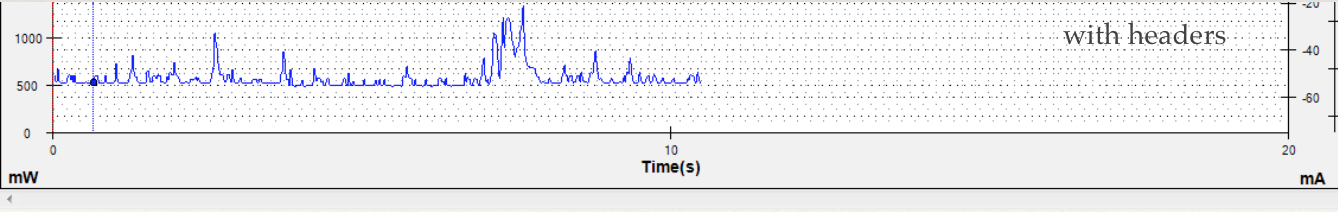
\includegraphics[width=80mm]{wifi_withheaders.png}
\caption{With Headers (Wifi) }
\label{fig:sp_gd_mnist}
\end{figure}

\bigskip

\subsection{Best Case}

In this more likely case, for a cached webpage with n resources, out of which m (m \textless \textless n) resources have been modified: regular HTTP makes {\it n} GET requests. Power-aware HTTP, on the other hand, makes {\it (1+m)} GET requests.

\subsection{Worst Case}

For a cached webpage with n resources, out of which all n resources have been modified, regular HTTP
makes {\it n} GET requests whle power-aware HTTP makes {\it (1+n)} GET requests.

The proposed solution cannot be used until all browsers provide the fucntionality to an HTTP GET request with the {\it check-reosurce} header. Standardization will thus ensure that the solution works across all browsers. Also, different hosting services can provide this functionality if a standard is established.

\bigskip

\section{More Optimizations}

We looked at some of the optimizations made by modern browsers. One of the optimizations done by Google Chrome to reduce latency is pre-fetching the URL before a user actually finishes typing the URL.
 
Server logs in the figure shows that  as  soon as user starts typing, Chrome starts making HTTP requests for each typed character. This approach reduces latency but consumes a lot of power and wastes a lot of network resources. 

\begin{figure}[ht!]
\centering
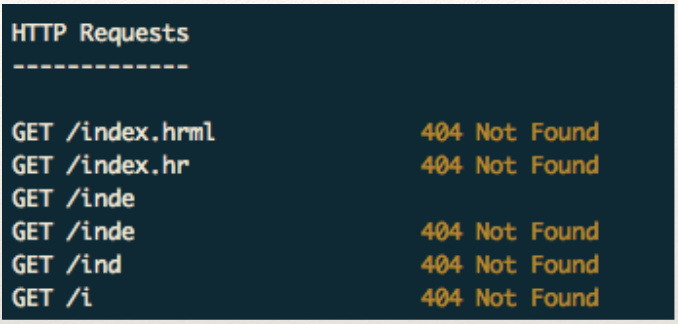
\includegraphics[width=80mm]{chrome}
\caption{Chrome URL Pre-Fetch}
\label{fig:sp_gd_mnist}
\end{figure}

We may try to tweak the response of 404 with possible URL options to save power i.e In a 404 request, it should be possible for a server to specify the possible set of urls matching the pattern. This could considerably reduce the power consumption and latency. Of course security needs to be taken into account but this could simply be a better layer of optimization instead of blindly making HTTP requests on the URL being typed. 

\bigskip

\section{ Related Works}

Other works that have proposed extensions similar to ours include the work on improving latency of HTTP by 22\% [1]. The authors propose two new HTTP request methods: GETALL and GETLIST to retrieve all the resources on a webpage with a single call. Our work differs in that we propose to have a cient query the server to check the resource change status and make subsequent GET requests for the modified resources based on the respnse from the server.

Another work suggests the use of a web proxy to reduce power consumption by not waiting for requests on a WAN and the use of request pipelining to reduce the wait period [2].

Google's SPDY project also mentions some strategies to reduce latency by 27\%[5]. SPDY fetches all requests in parallel. If an HTTP client has 4 connections per domain, and 20 resources to fetch, it would take roughly 5 RTs to fetch all 20 items. SPDY fetches all 20 resources in one RT. Our proposal however, is an extension to the HTTP protocol as it is implemented today and not a part of a larger solution.

\bigskip

\section{Conclusions}

Power consumption in a resource-constrained device depends on a number of factors. In our approach, we have targeted novel means to reduce the number of HTTP requests. In the implentation of HTTP today, all the resources on a cached webpage are fetched using different HTTP connections which increases the number of round trips. We propose an extension to HTTP to reduce the number of requests. The proposed solution shows clear quantitative gains in reducing power consumption over the existing implementation of HTTP. Also, the proposed solution need not modify the implementaion of existing servers; the change can be made at web proxies. We also highlighted the necessity of standardizing the extension.

\bigskip

\section{Future Work}

mutiple servers?

\bigskip

\section{References}

[1] Venkata N. Padmanabhan and Jeffrey C. Mogul ,Improving HTTP Latency \\[\baselineskip]
[2] Van Jacobson. Congestion Avoidance and Control. In Proc. SIGCOMM ’88 Symposium on Communications Architectures and Protocols, pages 314-329. Stanford, CA, August, 1988. \\[\baselineskip]
[3] Jon B. Postel. Transmission Control Protocol. RFC 793, Network Information Center, SRI International, September, 1981 \\[\baselineskip]
[4] Jen-yi Pan, Wei-Tsong Lee and Nen-Fu Huang, Indirect HTTP: An Energy Efficient Extension of Hypertext Transfer Protocol for Web Browsing \\[\baselineskip]
[5] SPDY: An experimental protocol for a faster web [White paper]. Retrieved from http://www.chromium.org/spdy/spdy-whitepaper

\end{document}





















	
